\section{Dobór parametrów}
\label{ch:parametry}

Przy implementacji filtru NLM pojawia się problem doboru parametrów algorytmu. Pierwszym parametrem jest $P$ określąjący maksymalną odległość próbki należącej do $\Delta$ od punktu $s$, a więc $L_\Delta=2P+1$. Dla sygnałów EKG odpowiednim wyborem dla $P$ jest liczba w okolicach połowy długości zespołu QRS.

\begin{figure}[!htb]
	\begin{center}
		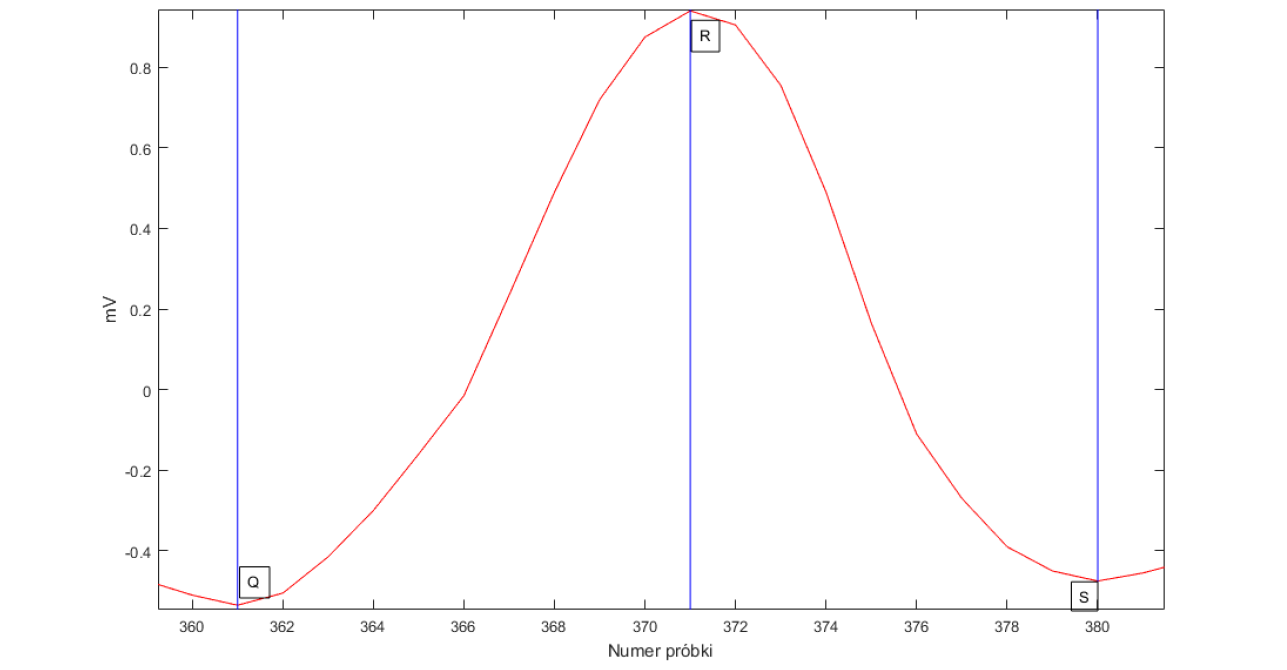
\includegraphics[width=15cm,clip]
		{img/qrs.png}
	\end{center}
	\caption{Fragment sygnału EKG zawierający zespół QRS. Sygnał pochodzi z Physionet MIT-BIH arrythymia database i jest oznaczony numerem 100.\cite{mitbih} }
	\label{rys:qrs}
\end{figure}
Z rysunku \ref{rys:qrs}. wynika, że odpowiednią wartością będzie $P=10$ próbek.

Parametr M reprezentuje połowę rozmiaru otoczenia $N(s)$ (czyli $|N(s)| = 2M+1$). Zapewnia on ,,mniej lokalne''  przeszukiwanie sygnału. Zakładając, że sygnał EKG jest praktycznie okresowy, im więcej ,,okresów'' zostanie uwzględnionych w obliczaniu estymaty $\hat{u}(s)$ tym lepsze wyniky powinno się uzyskać. Jednakże zbytnie zwiększenie obszaru poszukiwań powoduje dłuższe obliczenia. Przyjęto, że $M=2000$, a co za tym idzie, obszar poszukiwań obejmuje około 15 ,,okresów'' sygnału ECG.

Ostatnim, ale naistotniejszym parametrem jest pasmo $\lambda$, który odpowiada za wygładzenie estymaty zaszumionego sygnału EKG. Zbyt mała $\lambda$ powoduje złe dopasowanie wag przy uśrednianiu, zbyt duża wartość tego parametru skutkuje w traktowaniu niepodobnych do siebie fragmentów sygnału jako podobnych. Parametr ten zależy od wariancji $\sigma^2$ szumu i można przyjąć, że $\lambda=\frac{6}{10}\sigma$. Parametr ten został dobrany doświadczalnie, na bazie analizy zaszumionych przebiegów, wobec czego przyjęto, że $\sigma^2=0,0004$.\cite{tracey2012nonlocal}.